 
%%%%%%%%%%%%%%%%%%%%%%%%%%%%%%%%%%%%%%%%%%%
\documentclass[12pt]{report}	%Doccument Class Specification
\setlength{\textwidth}{6.25in} % original 6.25 %Text Lenght SetUp
\setlength{\textheight}{8in}
\renewcommand{\baselinestretch}{1.3}	%Page Margin SetUp
\oddsidemargin 20pt    %  Left margin on odd-numbered pages.
\evensidemargin 20pt   %  Note that \oddsidemargin = \evensidemargin
\topmargin 0pt
\newcommand{\squeezeup}{\vspace{-0.6cm}}
\renewcommand*\contentsname{INDEX}
%%%%%%%%%%%%%%%%%%%%%%%%%%%%%%%%%%%%%%%%%%%
\usepackage{amssymb}
\usepackage{amsmath}

\usepackage{algorithmic}


\usepackage {epsfig}
\usepackage{listing}
\usepackage {graphicx}
\usepackage{titlesec}
\usepackage{url}
\usepackage{fancyhdr}
\usepackage{float}
\usepackage{fancybox}
\usepackage{xcolor}
\usepackage[left=3.81cm,top=2.54cm,right=2.54cm,bottom=3.175cm]{geometry}
\usepackage{pdfpages}
\usepackage[font=normalsize,labelfont=bf]{caption}
\usepackage[]{hyperref}
\usepackage[intoc]{nomencl}

\usepackage{verbatim}
\makeindex
%%%%%%%%%%%%%%%%%%%%%%%%%%%%%%%%%%%%%%%%%%%
%Change Font Size Of Titles
\titleformat{\chapter}[display]
{\normalfont\Large\bfseries\centering}{\chaptertitlename\ \thechapter}{14pt}{\Large}
\titleformat{\section}{\Largesize \bfseries}{\thesection}{1em}{}
\titleformat{\subsection}{\Largesize \bfseries}{\thesubsection}{1em}{}
%%%%%%%%%%%%%%%%%%%%%%%%%%%%%%%%%%%%%%%%%%%
\begin{document}
	%%%%%%%%%%%%%%%%%%%%%%%%%%%%%%%%%%%%%%%%%%%	
	\fancypage{\setlength{\fboxsep}{10pt}\doublebox}{}	
		\begin{center}
		{ \large\bf  SYNOPSIS }\\
		\end{center} 

{\large\textbf{1: Group ID}}\\
{\small  Group number  30}\\


{\large\textbf{2: Project Title}}\\
{\small  "High Speed Data Communication using LiFi providing Security"}\\


{\large\textbf{3: Project Option}}\\
{\small Internal Project }\\


{\large\textbf{4: Internal Guide}}\\
{\small Prof. Anuja Bharate} \\


{\large\textbf{5: Sponsorship}\\
{\small N/A}\\


{\large\textbf{6:  Technical Keywords }\\
{\small 1.C. Computer Systems Organization  
        \newline C.2 Computer Communication Networks
        \newline C.2.1 Network Architecture and Design
       \= \newline A. Wireless Communication
        \newline B. Distributed Networks 
        \newline
       }\\
        
        
{\large\textbf{7: Problem Statement}\\
{\small "To overcome the Limitations of existing LiFi technology and to provide secure and easy to use communication between various devices."}
\newline\\


{\large\textbf{8: Abstract }\\
{\small \paragraph{}The proposed system demonstrates transmission and reception of data by switching LED ON and OFF at very high intensity which is too fast to be noticed by human eyes.  A system which will use this LED blink data transmission technique and allow us to transmit data over various devices for which it is necessary to  develop a LiFi based data transmission technique which will provide higher data transmission speed with data security and easy to use communication technology.}\\


{\large\textbf{9: Goals And Objective}\\
{\small          1) To provide better data transmission technologies to the Modern Computing devices.
       {\newline 2) High Speed}
       {\newline 3) To Manage LiFi Powered Devices.}
       {\newline 4) Provide LiFi to Mobile and Stationary Computing Devices.}\\
       
       
{\large\textbf{10: Relevant mathematics associated with the Project}\\
{\small  System Description:
	{\newline •	Input: Reading a file or text input from user.}
	{\newline •	Output: Provide requested  data to  user.}
	{\newline Success Conditions: Successful data transmission using VLC without interrupts}
	{\newline •	Failure Conditions: Data interruption, data loss, data unavailability, etc.}
	\\
	\\
	S = \{I, O, F, S \}
	\newline Where,
	\newline I= Input from the user in text format or input as a file
	\newline O= Given text or a file at receiver side
	\newline F= Failure condition
	\newline S= Success condition}\\



{\large\textbf{11: Names of Conferences / Journals where papers
can be published}\\
{\small  1.IJCA Publications 
\newline 2.SPPU Publication
\newline 3.IEEE/ACM
\newline
      }\\
       
       
{\large\textbf{12: Review of Conference/Journal Papers supporting Project idea}\\

{\small
References: 
\newline \textbf{ 1) "High sensitivity universal LiFi receiver for enhanced data communication"}\\
\textbf{Authors:} Zashi P. Chaudhari, Satish R. Devane\\
\textbf{Description: }In todays world communication between the devices is much common. Radio wave spectrum is very small part of spectrum available for communication but with increase in advanced technology and number of users the network becomes overloaded which results in failure to provide high data rate. Visible light acts as rival to the present wireless radio frequency communication by larger bandwidth and high data rate.\\
\textbf{DOI: }10.1109/GET.2016.7916619\\
\textbf{Year: }2016\\
\newline \textbf{ 2) "LiFi – The path to a New Way of Communication"}\\
\textbf{Authors:} Monica Leba, Simona Riurean, Andreea Lonica\\
\textbf{Description: }Important research efforts have been directed over the past ten years, towards exploring alternative parts of thee electromagnetic spectrum that could potentially offload a large portion of the network traffic from the overcrowded radio frequency(RF) domain. This paper summarizes most of the research , developments and application achieved so farand looks at the different aspects of the strengths and weaknesses, implementations, challenges, VLC IEEE standard and modulation technique of the VLC and specific LiFi's new coined optical wireless communication technology.\\
\textbf{DOI: }10.23919/CISTI.2017.7975997\\
\textbf{Year: }2017\\
\newline \textbf{3)  "Integrated LiFi (Light Fidelity) for smart communication through illumination"}\\
\textbf{Authors:}R. Mahendran\\
\textbf{Description: }The intensity of the LEDs is varied by  alternating the current passed through them at very high speeds. However, the human eye cannot recognize this change and the LEDs appear to have a constant intensity. This ON-OFF activity of LED lights facilitate data transmission using binary codes i.e, when the LED is ON, logical1'1' is transmitted and when the LED OFF, logical '0' is transmitted.\\ 
\textbf{DOI: }10.1109/ICACCCT.2016.7831599\\
\textbf{Year: }2016\\
\newline \textbf{4)  "LiFi: Conceptions, misconceptions and opportunities"}\\
\textbf{Authors: }Harald Hass\\
\textbf{Description: }In this talk we will first explain what Light Fidelity(LiFi) is and highlight the key differences to visible light communication(VLC). We will discuss misconception and illustrate the potential impact this technology can have across a number of existing and emerging industries.\\
\textbf{DOI: }10.1109/IPCon.2016.7834279\\
\textbf{Year: }2016\\
\newline \textbf{5)  "Future internet and Internet of things"}\\
\textbf{Authors: }Pradeep Kumar\\
\textbf{Description: }The future Internet will be capable of connecting and communicating with almost all physical and virtual objects around us to the existing Internet. The Internet of Things is a vision that entails connectivity among different physical and virtual objects in order to understand how the life would change when things, homes and cities become smart.\\
\textbf{DOI: }10.1109/ICIEECT.2017.7916594\\
\textbf{Year: }2017\\
\newline \textbf{6) "Prototyping and measurements for a LiFi system"}\\
\textbf{Authors: }Kun Chen Hu\\
\textbf{Description: }The prototype is based on two Spartan 6 FPGAs and uses a Light Emitting Diode (LED) to transport the information through amplitude changes of the light. The receiver uses a low dark current PIN photodiode. We describe the system design, the receiver algorithms and the measurement set-up. We present some measurements where in a Line of Sight (LOS) channel the received pulses are shown to match the transmitted ones.\\
\textbf{DOI: }10.1109/SAM.2016.7569701\\
\textbf{Year: }2016\\
\newline \textbf{7) "Digital data transmission via visible light communication(VLC): Application vehicle to vehicle communication"}\\
\textbf{Authors: }Dahmani Mohammed\\
\textbf{Description: }Visible Light Communication(VLC) may improve driver's safety by allowing the vehicles to communicate easily with each other (V2V communication). The first prototype of an unidirectional VLC communication was developed at the laboratory of signals and images (LSI) of USTO-MB. The experimental results are more than satisfactory.\\
\textbf{DOI: }10.1109./CEIT.2016.7929059\\
\textbf{Year: }2016\\
\newline \textbf{8) "Impact of VLC on Light Immission Quality of White LEDs"}\\
\textbf{Authors: }Wasiu O. Popoola\\
\textbf{Description: }This paper reports the effect of data modulation on the emitted light quality of phosphor converted white LEDs. The results showed that provided the expected average current driving the LEDs remains unchanged then the emitted light quality will stay the same. For a dc-balanced modulating signal, with a nonvarying average value, any fluctuations in the instantaneous driving current due to data modulation do not have any significant impact on the measured light quality metrics. \\
\textbf{DOI: }10.1109/JLT.2016.2542110\\
\textbf{Year: }2016\\
\newline \textbf{9) "On visible light communication and quality of light emitted from illumination LEDs"}\\
\textbf{Authors: }Wasiu O.Popoola\\
\textbf{Description: }We present the effect of LiFi, with on-off keying modulation technique, on the quality of light emitted from LEDs. Findings show that to preserve the LED light quality, the LiFi data signal should be such that the LED average drive current remains unchanged.\\
\textbf{DOI: }10.1109/PHOSST.2016.7548765\\
\textbf{Year: }2016\\
  
{\large\textbf{13. Plan of Project Execution}}\\
\begin{figure}[ht]
	\centering
	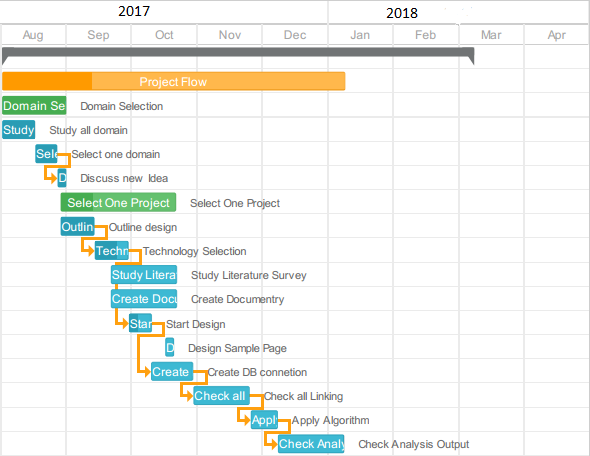
\includegraphics[width=6in]{plan.png}
	\begin{center}\caption{Plan of Project Execution} \end{center}
	\label{LABEL}
\end{figure}
\end{document}
	
